\documentclass{article}
\usepackage{fullpage}
\usepackage{amsmath,amsfonts,amssymb,graphicx}
\usepackage[mathscr]{eucal}
\usepackage{stmaryrd}
\usepackage{amsbsy}
\usepackage{bm}
\usepackage[usenames]{color}
\usepackage[dvipsnames]{xcolor}
\usepackage{parskip} 
\usepackage{natbib}
\usepackage{comment}
%% For \subfloat command
\usepackage{subfig}

\newcommand{\fixme}[1]{{\color{red}\textbf{#1}}}
\newcommand{\T}[1]{\boldsymbol{\mathscr{\MakeUppercase{#1}}}} %tensor

%% Shorthand for Real
\newcommand{\Real}{\mathbb{R}}

\newcommand{\tr}{\operatorname{tr}} % Trace
\newcommand{\Kron}{\otimes} %Kronecker


\newcommand{\E}{\mathrm{E}}
\newcommand{\Cov}{\mathrm{Cov}}
\newcommand{\Corr}{\mathrm{Corr}}
\newcommand{\Ehat}{\hat{\E}}
\newcommand{\Covhat}{\hat{\Cov}}
\newcommand{\vect}{\mathrm{vec}}
\newcommand{\vech}{\mathrm{vech}}
\newcommand{\indep}{\;\, \rule[0em]{.03em}{.6em} \hspace{-.25em}
\rule[0em]{.65em}{.03em} \hspace{-.25em}
\rule[0em]{.03em}{.6em}\;\,}
\newcommand{\rank}{\mathrm{rank}}
\newcommand{\real}[1]{\Real \mathit{^{#1}}}
\newcommand{\trans}{^{\mbox{\tiny {\sf T}}}}
%\newcommand{\itrans}{^{\mbox{-\tiny {\sf T}}}}
\newcommand{\spn}{\mbox{span}}
\newcommand{\spc}{{\mathcal S}}
\newcommand{\diag}{\mathrm{diag}}
\newcommand{\cs}{\spc_{Y|\Xbf}}
\newcommand{\Var}{\mathrm{Var}}

%% Vectors
\newcommand{\V}[1]{{\bm{\mathbf{\MakeLowercase{#1}}}}} % vector
\newcommand{\VE}[2]{\MakeLowercase{#1}_{#2}} % vector element
\newcommand{\Vbar}[1]{{\bm{\M{A}r \mathbf{\MakeLowercase{#1}}}}} % vector
\newcommand{\Vhat}[1]{{\bm{\hat \mathbf{\MakeLowercase{#1}}}}} % vector
\newcommand{\Vtilde}[1]{{\bm{\tilde \mathbf{\MakeLowercase{#1}}}}} % vector
\newcommand{\Vn}[2]{\V{#1}^{(#2)}} % n-th vector
\newcommand{\VnE}[3]{{#1}^{(#2)}_{#3}} % n-th vector
\newcommand{\VtildeE}[2]{\tilde{\MakeLowercase{#1}}_{#2}} % vector element


%% Matrices
\newcommand{\Tra}{^{\sf T}} % Transpose
\newcommand{\M}[1]{{\bm{\mathbf{\MakeUppercase{#1}}}}} % matrix
\newcommand{\ME}[2]{\MakeLowercase{#1}_{#2}} % matrix element
\newcommand{\MC}[2]{\V{#1}_{#2}}
\newcommand{\Mr}[2]{\V{#1}_{#2}} % matrix row
\newcommand{\Mhat}[1]{{\bm{\hat \mathbf{\MakeUppercase{#1}}}}} % matrix
\newcommand{\Mtilde}[1]{{\bm{\tilde \mathbf{\MakeUppercase{#1}}}}} % matrix
\newcommand{\MhatC}[2]{\Vhat{#1}_{#2}} % matrix column
\newcommand{\Mbar}[1]{{\bm{\bar \mathbf{\MakeUppercase{#1}}}}} % matrix
\newcommand{\MbarC}[2]{\Vbar{#1}_{#2}} % matrix column
\newcommand{\Mn}[2]{\M{#1}^{(#2)}} % n-th matrix
\newcommand{\Mbarn}[2]{\Mbar{#1}^{(#2)}} % n-th matrix
\newcommand{\Mtilden}[2]{\Mtilde{#1}^{(#2)}} % n-th matrix
\newcommand{\MnTra}[2]{\M{#1}^{(#2){{\sf T}}}} % n-th matrix transpose
\newcommand{\MnE}[3]{\MakeLowercase{#1}^{(#2)}_{#3}} % n-th matrix element
\newcommand{\MnC}[3]{\V{#1}^{(#2)}_{#3}} % n-th matrix column
\newcommand{\MbarnC}[3]{\Vbar{#1}^{(#2)}_{#3}} % n-th matrix column
\newcommand{\MnCTra}[3]{\V{#1}^{(#2){{\sf T}}}_{#3}} % n-th matrix column transpose
\newcommand{\MCTra}[2]{\V{#1}^{{\sf T}}_{#2}} % n-th matrix column transpose
\newcommand{\prox}{\mathop{\rm prox}\nolimits}
\newcommand{\Pcal}{{\mathcal{P}}}
\newcommand{\greekbold}[1]{\mbox{\boldmath $#1$}}
\newcommand{\Sigmabf}{\greekbold{\Sigma}}


%% For comments to each other
\newcommand{\Remark}[2]{{\color{red}Remark from #1: #2}}
\newcommand{\Note}[1]{{{\color{red}{#1}}}}

\newcommand{\Eric}[2]{{\bf {\color{MidnightBlue}@Eric from #1: #2}}\xspace}
\newcommand{\Joe}[2]{{\bf {\color{Plum}@Joe from #1: #2}}\xspace}
\newcommand{\Halley}[2]{{\bf {\color{OliveGreen}@Halley from #1: #2}}\xspace}
\newcommand{\All}[2]{{\bf {\color{Sepia}@All from #1: #2}}\xspace}


\begin{document}
\title{Baseline Drift Estimation for Air Quality Data Using Quantile Trend Filtering}
\author{}
\date{}
\maketitle

\section*{General Remarks}

We thank the referees for their useful feedback and believe the manuscript is improved as a result. 

In our revision we have denoted in \color{red}red \color{black} substantial newly added text. For the sake of readability we did not highlight minor edits in the revision.
Finally, we give point-by-point responses to referee comments below.
%\section*{Editor}
%
%\begin{quote}


%\Note{Should we mention here that we address reviewer 2's comments in the file?}
%
%\end{quote}

%\section*{Associate Editor}

\section*{Reviewer 1}

\begin{comment}
Authors present a method for quantile trend filtering with a non-crossing constraint. 
The use the ADMM algorithm to reduce the computing time. 
They compare their method with other approaches by numerical experiments. 
Finally, their approach is used on real data.

I really enjoy the paper. The method is interesting and well introduced. The approach requires different tuning parameters and I think that the choice of these parameters should be more discussed (see my comments below).

Major comments:
- The approach implies different tuning parameters: the penalty $\lambda$, the number of windows $W$, the bounds of the windows (l_w, u_w) and the degree of the polynomials (k). The selection of $\lambda$ is well described in Section 3. However, how the number of windows and the bounds of the windows are selected? In the paper, the degree of polynomials is k=2. Can the information criteria introduced in Section 3 be used to estimate k?

- In Section 3.1, authors said that the method can easily handle missing data. What are the assumption on the process of randomness (MAR, MCAR,...)?

- In Section 3.2, the BIC is introduced. I'm agree that for Bayesian quantile regression, the asymmetric Laplace likelihood is generally used. Does the choice of $\sigma$ impact the results? Moreover, in a Bayesian framework, a penalized regression can often be defined with a specific prior distribution on the parameters (L1-type regression can be defined by using a Laplace distribution as prior). Is it possible to define such prior for the problem defined by Equation (10)?

Minor comments:

- At the end of Section 3.2, maybe more details should be given about the properties of the eBIC for the large parameter spaces (is it more efficient than the BIC)?

- Figure 7,8 and 10 are not really clear. May be they can be replaced by tables.

\end{comment}

1. The approach implies different tuning parameters: the penalty $\lambda$, the number of windows $W$, the bounds of the windows $(l_w, u_w)$ and the degree of the polynomials $(k)$. The selection of $\lambda$ is well described in Section 3. However, how the number of windows and the bounds of the windows are selected? 

\begin{quote}
The referee raises a good question. Our motivation for casting the problem as a linked set of estimations over overlapping windows is computational. Ideally there would be just one window to estimate the trend over, rather than $W > 1$ but as the trends in the timing experiments in Figure~5 indicate, using a single window will become computationally impractical if one wishes to fit a model over a very large set of time points. Our numerical experiments show a little less than a linear speed up in the number of windows used. Thus, if one wished to cut the overall running time to fit a family quantile trends by a roughly factor of 10, one would choose in the ballpark of 11 or 12 windows. The bounds of the windows and amount of overlap between windows depends on the application and should be larger than the expected time duration of transient events. We have added additional sentences addressing these points in the revised manuscript at the end of Section 2.
\end{quote}

2. In the paper, the degree of polynomials is $k=2$. Can the information criteria introduced in Section 3 be used to estimate $k$?

\begin{quote}
The expected degrees of freedom in the standard trend-filtering problem is given by the number of knots in $\V{\theta}$ plus $k+1$ \citep{Tib2014}. Consequently, a natural strategy to estimate $k$ is to use the eBIC criterion introduced in Section 3 but with $\nu$ equal to the number of knots in $\V{\theta}$ plus $k+1$. We have added additional sentences addressing these points in the revised manuscript at the end of Section 3.
\end{quote}

3. In Section 3.1, authors said that the method can easily handle missing data. What are the assumption on the process of randomness (MAR, MCAR,...)?

\begin{quote}
This is a good question. It turns out the penalized negative log-likelihood in Section 3.1 corresponds to making a MCAR assumption. We've added a short discussion of this in Section 3.1.
\end{quote}

4. In Section 3.2, the BIC is introduced. I'm agree that for Bayesian quantile regression, the asymmetric Laplace likelihood is generally used. Does the choice of $\sigma$ impact the results? 

\begin{quote}
We did not find that the choice of $\sigma$ affected the results. The following figure plots the eBIC criteria against $\sigma$ for an example dataset. The value of $\lambda$ chosen is the same for all values of $\sigma$ compared, but the $\sigma$ used in the analysis (0.1) results in a eBIC value that rises more rapidly after achieving the minimum. 

\begin{figure}[h!]
\centering
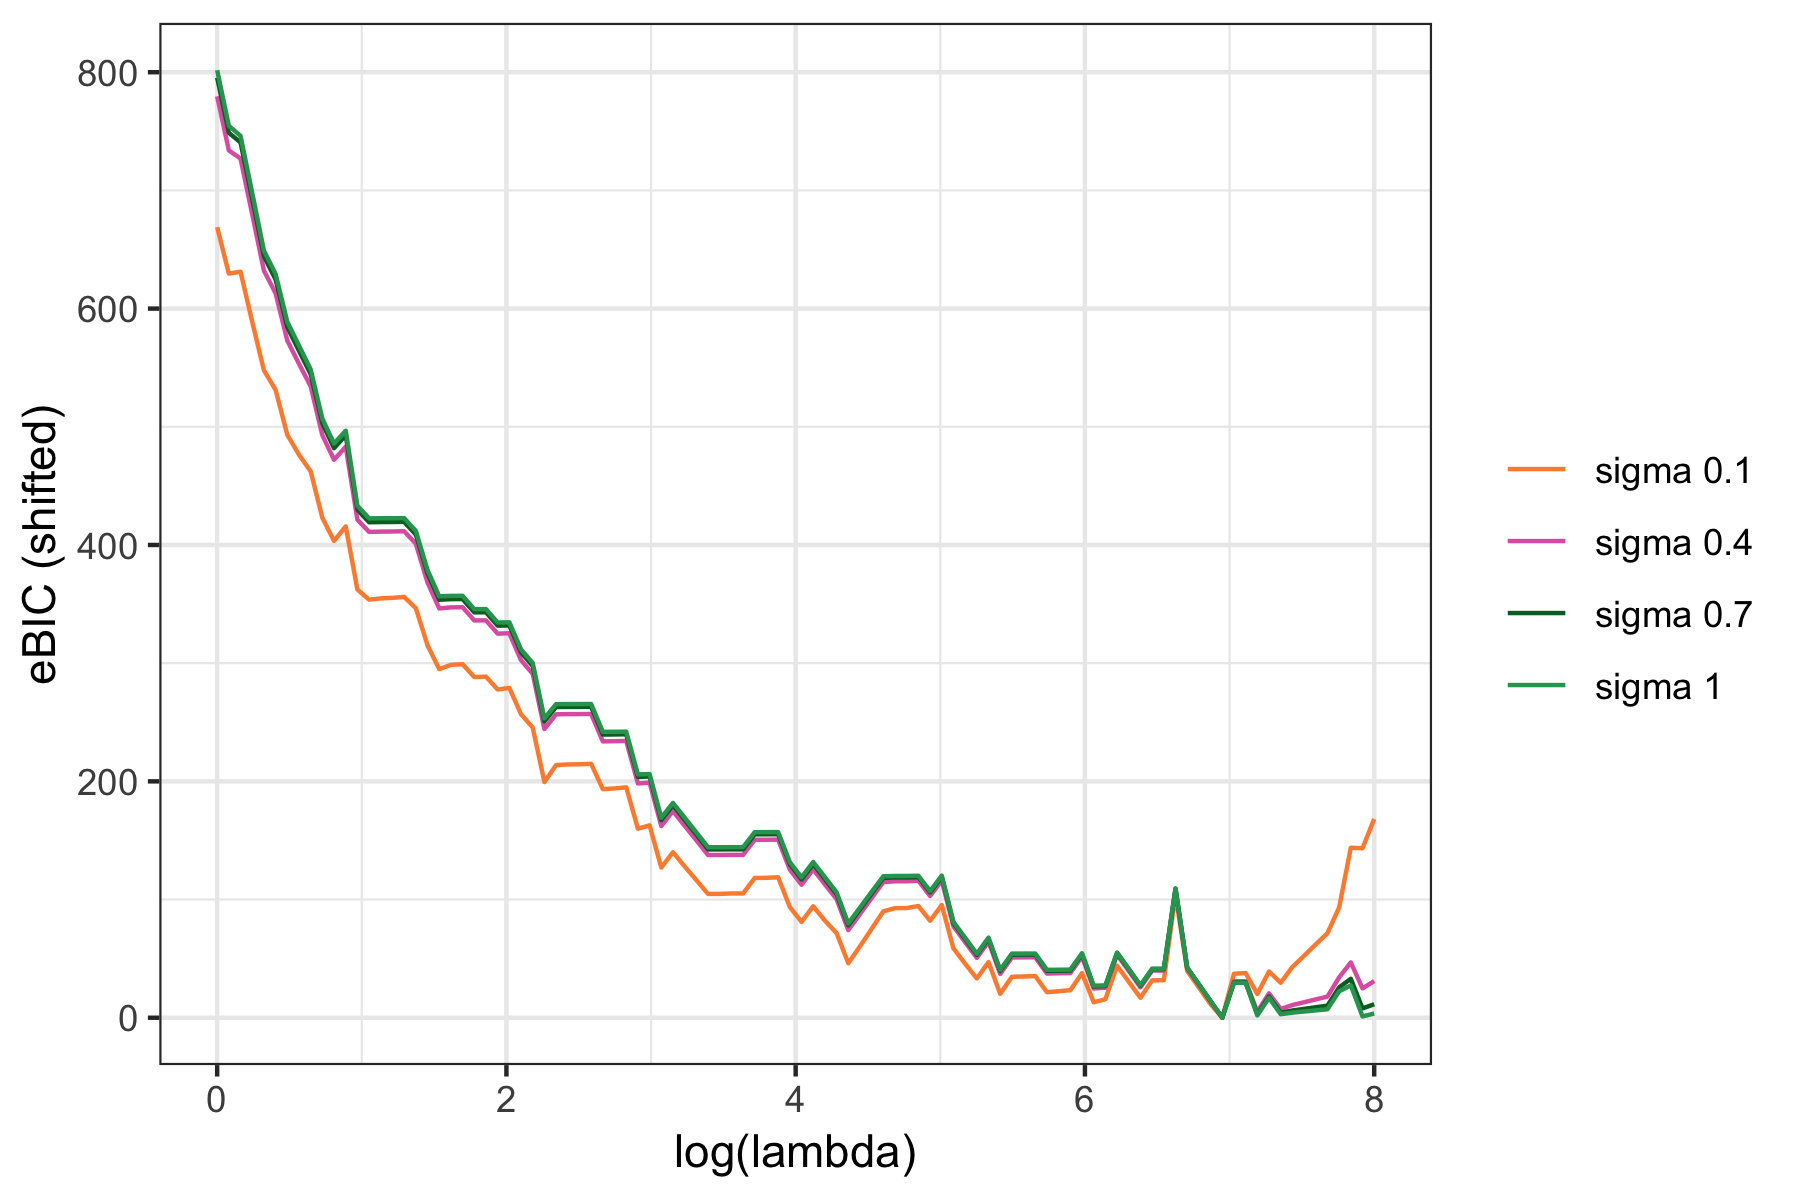
\includegraphics[width = 0.7\linewidth]{BIC_by_lambda_and_sigma.png}
\end{figure}
\end{quote}

5. Moreover, in a Bayesian framework, a penalized regression can often be defined with a specific prior distribution on the parameters (L1-type regression can be defined by using a Laplace distribution as prior). Is it possible to define such prior for the problem defined by Equation (10)?

\begin{quote}
Yes it is possible to define such a prior for the probelm defined by Equation (10). \cite{faulkner2018locally} proposed a few fully Bayesian variations of the trend filter utilizing shrinkage priors on the $k$th-order differences in values of the unknown target function. They used a Gaussian likelihood for the data corresponding to the squared loss used by \cite{Kim2009}. A fully Bayesian variation of the quantile trend filter could be implemented by substituting the Laplace likelihood for the Gaussian likelihood. %We have added these points to the discussion of prior work. 
We have added these points in the revised discussion.
\end{quote}

\subsection*{Minor comments:}

6. At the end of Section 3.2, maybe more details should be given about the properties of the eBIC for the large parameter spaces (is it more efficient than the BIC)?

\begin{quote}
Thank you for the suggestion. The eBIC has been proven to be model selection consistent in cases where the BIC can be model selection inconsistent. This difference between the eBIC and BIC manifests itself practically in the trend filtering problem in that the BIC selected models tend to be undersmoothed in comparison to the eBIC selected models. We have added sentence highlighting these advantageous properties of the eBIC for large parameter spaces in Section 3.2.

%``A limitation of the BIC, however, is that it may be inconsistent in the high-dimensional setting. This issue arises as a consequence of an implicit assumption in deriving the BIC that all models under consideration are equally likely. Consequently, in the context of variable selection methods such as the lasso, models that include more covariates (up to half of all possible covariates) will have a larger prior probability of being selected under the BIC criterion. In the context of this work, using the BIC may have a tendency to favor the selection of undersmoothed signals, as signals $\V{\theta}$ with more non-zero entries in the vector  $\Mn{D}{k+1}\V{\theta}$ will be assigned higher prior probabilities under the BIC.

%To address this issue, \cite{chen2008} modified the prior probabilities to dampen the prior weight on larger models, or in the context of this work, undersmoothed signals, and proposed 
%... They prove that the eBIC is model selection consistent under mild regularity conditions."
\end{quote}

7. Figure 7,8 and 10 are not really clear. May be they can be replaced by tables.

We have added tables with the results to the supplemental materials but feel that they are too long to include in the manuscript itself. 

\section*{Reviewer 2}

\begin{comment}
The paper address the issue of estimating multiple quantile trends simultaneously in time series data. This problem is common in several fields from economics to medicine. The authors focused on the application to low cost air quality sensor. Thus the paper fits with AOAS policy. However, to improve the suitability, I suggest the authors to add more on how to employ their model and algorithm to data beyond to the application presented and which specific question this algorithm can address in different disciplines. While the problem to be addressed is clearly explained, the introduction miss a broader presentation of the topic to attract Statistician readers from differ fields. The authors claim that demixing problems is common to different applications with some references, thus they should comment more on this and reinforce the interest of the paper. Part of the technical material on the ADMM algorithm should be moved to appendices or online supplements.

The paper is correct. The algorithm is tested on simulated and real data supporting the validity of the results. The methodology and the results are well supported by figures and comments all over the test. Authors should check some typos spread in the manuscript.

Overall, the paper is sounds and interesting. It will benefit the community of Statistician working on low cost sensor data, an extremely increasing community. It will be of inspiration for scientists working with time series.
\end{comment}

The paper address the issue of estimating multiple quantile trends simultaneously in time series data. This problem is common in several fields from economics to medicine. The authors focused on the application to low cost air quality sensor. Thus the paper fits with AOAS policy. 

8. However, to improve the suitability, I suggest the authors to add more on how to employ their model and algorithm to data beyond to the application presented and which specific question this algorithm can address in different disciplines. While the problem to be addressed is clearly explained, the introduction miss a broader presentation of the topic to attract Statistician readers from differ fields. The authors claim that demixing problems is common to different applications with some references, thus they should comment more on this and reinforce the interest of the paper. 

\begin{quote}
We have expanded our discussion of baseline trend filtering applications to include electrocardiogram data, electrooculographic data, mass spectrometry, chromatography, macroeconomics, environmental science, laser-induced breakdown spectroscopy, and astronomy. We have also included one or more references for each example that requires baseline removal. These additions have been made on page 2 of the revision. We have also added a short paragraph at the end of the Section 6 on how our proposed method could potentially be used more generally for robust smoothing of time series data.
%\All{Eric}{Joe and Eric take lead in addressing, but please add any thoughts, Halley.} More applications: mass spec \cite{Du2006}. We don't explore it in this paper but we could use the framework for performing robust trend filtering by focusing on the quantiles close to the median. This might be useful for separating financial time series data into smooth trends and removing transient ups and downs. Maybe add this last observation to the discussion.
\end{quote}

9. Part of the technical material on the ADMM algorithm should be moved to appendices or online supplements.

\begin{quote}
We have moved part of the technical details of the ADMM algorithm to the supplementary materials.
\end{quote}

10. Authors should check some typos spread in the manuscript.

\begin{quote}
Thank you. We have checked and corrected for typos.
\end{quote}

\bibliographystyle{plainnat}
\bibliography{detrendify}
\end{document}